 %%%%%%%%%%%%%%%%%%%%%%%%%%%%%%%%%%%%%%%%%
% Developer CV
% LaTeX Template
% Version 1.0 (28/1/19)
%
% This template originates from:
% http://www.LaTeXTemplates.com
%
% Authors:
% Jan Vorisek (jan@vorisek.me)
% Based on a template by Jan Küster (info@jankuester.com)
% Modified for LaTeX Templates by Vel (vel@LaTeXTemplates.com)
%
% License:
% The MIT License (see included LICENSE file)
%
%%%%%%%%%%%%%%%%%%%%%%%%%%%%%%%%%%%%%%%%%

%----------------------------------------------------------------------------------------
%	PACKAGES AND OTHER DOCUMENT CONFIGURATIONS
%----------------------------------------------------------------------------------------

\documentclass[9pt]{developercv} % Default font size, values from 8-12pt are recommended

%----------------------------------------------------------------------------------------

\begin{document}

%----------------------------------------------------------------------------------------
%	TITLE AND CONTACT INFORMATION
%----------------------------------------------------------------------------------------

\begin{minipage}[t]{0.14\textwidth} % 45% of the page width for name
	\vspace{-\baselineskip} % Required for vertically aligning minipages
	
	% If your name is very short, use just one of the lines below
	% If your name is very long, reduce the font size or make the minipage wider and reduce the others proportionately
%\colorbox{black}{{\huge\textcolor{white}{\textbf{\MakeUppercase{Cesar Ochoa}}}}} % First name
\begin{tikzpicture}
    \clip (-0.5,-1.75) rectangle +(2.1cm,2.1cm);
    
    \node at (0,-.75) {\includegraphics[width = 3cm]{img/scotland_far.JPG}};
    %\clip (-1.5,-2.4) rectangle +(2cm,2cm);
    
    %\node at (0,-.75) {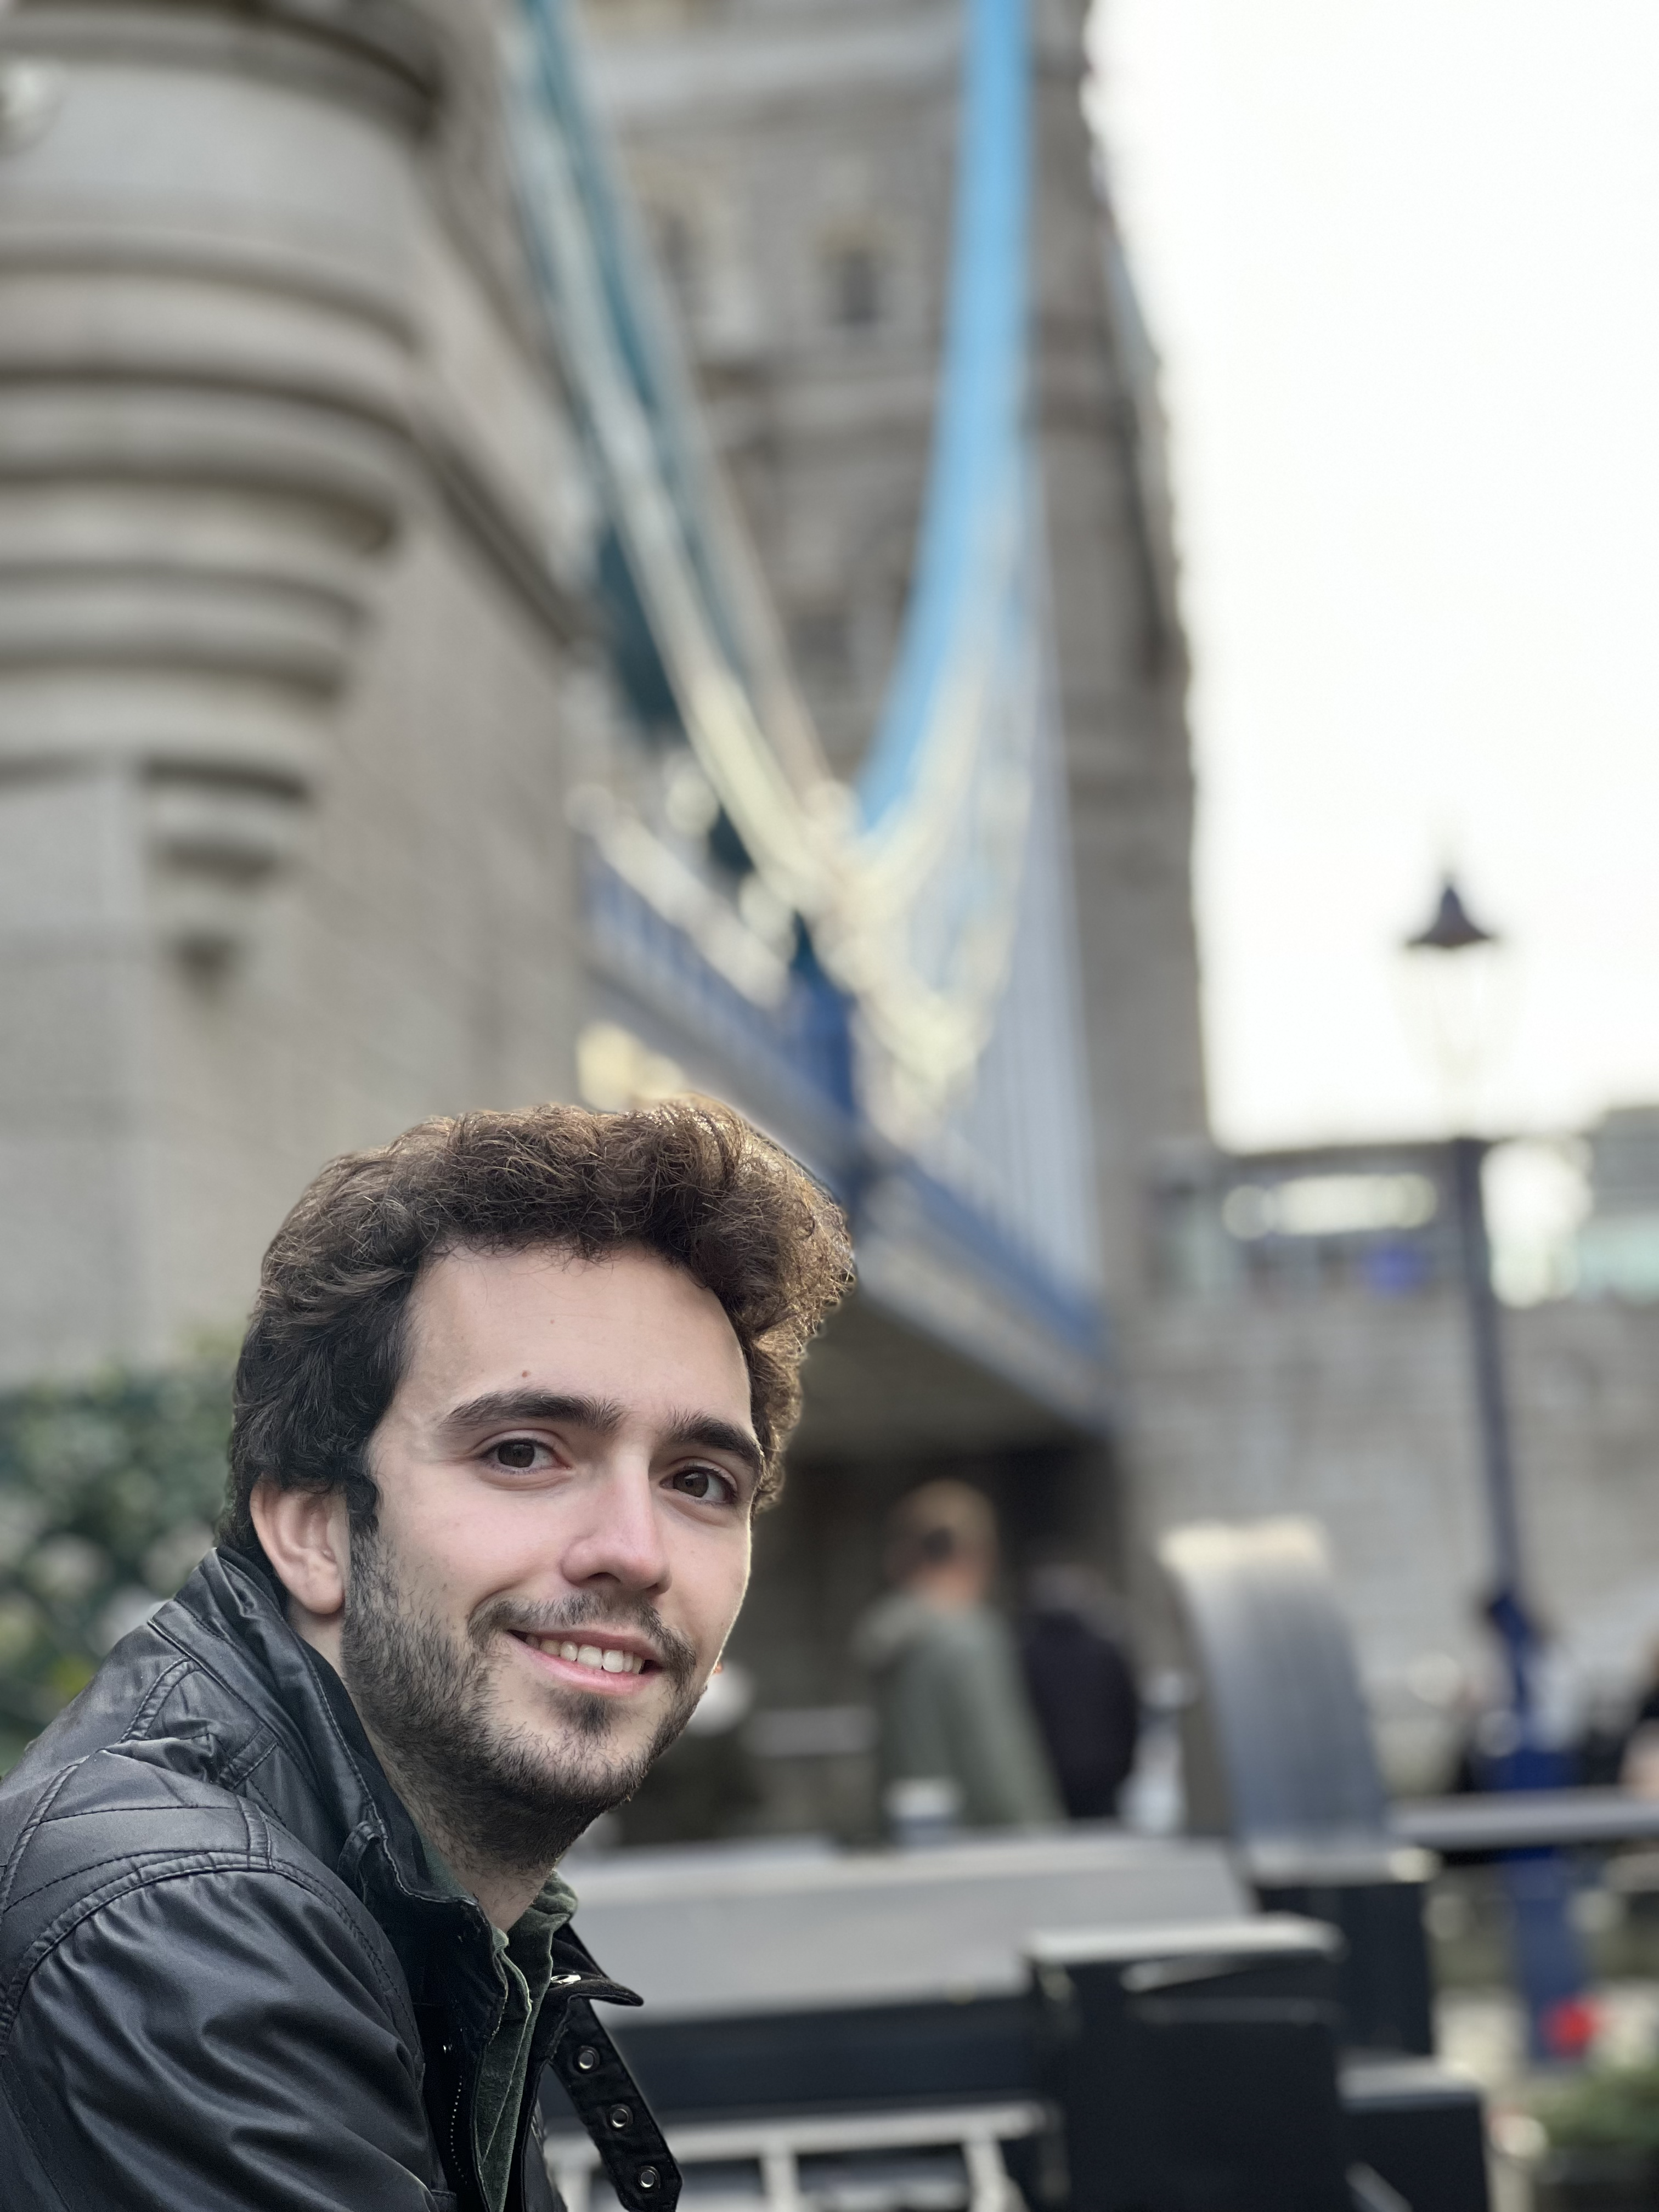
\includegraphics[width = 3cm]{img/london.png}};
    % if necessary the picture may be moved by changing the at (coordinates)
    % width defines the 'zoom' of the picture
\end{tikzpicture}
\end{minipage}
\begin{minipage}[t]{0.56\textwidth} % 45% of the page width for name
	\vspace{-\baselineskip}
	\fontsize{24}{26}{\textbf{Cesar Ochoa}}% First name
	
%	\colorbox{black}{{\textcolor{white}{\textbf{\MakeUppercase{Ochoa}}}}} % Last name
	
	\vspace{6pt}
	
	\large \textbf{AI Engineer}, Grupo Oesía\\
 \textbf{MSc Design Informatics}, The University of Edinburgh\\
\textbf{BSc Mathematics}, The University of Manchester% Career or current job title
\end{minipage}
\begin{minipage}[t]{0.30\textwidth} % 27.5% of the page width for the first row of icons
	\vspace{-\baselineskip} % Required for vertically aligning minipages
	\begin{flushright}
	\vspace{5pt}
	% The first parameter is the FontAwesome icon name, the second is the box size and the third is the text
	% Other icons can be found by referring to fontawesome.pdf (supplied with the template) and using the word after \fa in the command for the icon you want
	
	%\icon{MapMarker}{12}{Flat 48, 117 Hornsey Lane, London, N6 5NW}\\
	\icon{Phone}{12}{+44 792 393 6908}\\
	\icon{At}{12}{\href{mailto:caeochoa@gmail.com}{caeochoa@gmail.com}}\\
    \icon{Linkedin}{12}{\href{https://www.linkedin.com/in/caeochoa/}{/in/caeochoa}}\\
    
   % \large{Manchester}\\
    %\large{+44 (0) 792 393 6908}\\
    %\large{caeochoa@gmail.com}\\
    \end{flushright}
\end{minipage}
%\begin{minipage}[t]{0.275\textwidth} % 27.5% of the page width for the second row of icons
%	\vspace{-\baselineskip} % Required for vertically aligning minipages
	
	% The first parameter is the FontAwesome icon name, the second is the box size and the third is the text
	% Other icons can be found by referring to fontawesome.pdf (supplied with the template) and using the word after \fa in the command for the icon you want
%	\icon{Linkedin}{12}{\href{https://www.linkedin.com/in/caeochoa/}{/in/caeochoa}}\\
%\end{minipage}

\vspace{0.5cm}

%----------------------------------------------------------------------------------------
%	INTRODUCTION, SKILLS AND TECHNOLOGIES
%----------------------------------------------------------------------------------------
%----------------------------------------------------------------------------------------
%	EXPERIENCE
%----------------------------------------------------------------------------------------
%----------------------------------------------------------------------------------------
%	add list of skills as tags, highlighting the most relevant ones for each job?
%----------------------------------------------------------------------------------------


\cvsect{Work experience}

\begin{entrylist}
	
\bentry
{2024 -- present}
{AI Engineer}
{Grupo Oesía}
{\begin{itemize}
    \item{Led backend development of OKM, a no-code RAG platform for enterprises. Implemented document QA, SQL query translation, and multi-step reasoning agents with self-validation capabilities.}
    \item{Led computer vision module improvement for Banco-IR, a real-time object detection project. Reduced latency to <20ms through ONNX/CUDA optimization and model retraining. Mentored a junior developer through systematic knowledge transfer, resulting in successful project handover and improved client satisfaction.}
\end{itemize}

\texttt{Python}\slashsep\texttt{LangChain}\slashsep\texttt{PyTorch}\slashsep\texttt{ONNX}\slashsep\texttt{CUDA}\slashsep\texttt{Azure}\slashsep\texttt{SQL}}
            
\bentry
{2022 -- 2024}
{Technical Business Analyst}
{Acturis}
{\begin{itemize}
    \item{Led and managed over 20 projects end-to-end, handling client relationships through weekly meetings, overseeing website operations for major clients, and translating complex requirements into technical specifications across multiple platforms.}
    \item{Demonstrated rapid autonomous learning by mastering complex technical systems and insurance industry software, ensuring seamless project transitions and efficient knowledge transfer to stakeholders.}
\end{itemize}

\texttt{HTML}\slashsep\texttt{CSS}\slashsep\texttt{Javascript}\slashsep\texttt{React}\slashsep\texttt{SQL}}

        \bentry
		{2022 -- 2023\\\footnotesize{part time}}
		{Developing the Vision Checklist}
		{The University of Edinburgh}
		{\begin{itemize}
		    \item Continued collaboration with the University of Edinburgh post-dissertation to enhance and expand the Python-based Vision Checklist, improving its functionality for computer vision AI tests and user accessibility.
		\end{itemize}
		\texttt{Python}\slashsep\texttt{Computer Vision}\slashsep\texttt{Matplotlib}\slashsep\texttt{NumPy}}

         % \bentry
	%	{2018 -- 2019\\\footnotesize{part time}}
	%	{Design Assistant}
	%	{7billionideas}
	%	{\begin{itemize}
	%	    \item Designed and produced a range of educational and marketing materials, leveraging tools like Adobe Suite, Microsoft Office, WordPress, and Mailchimp, while coordinating remotely with an office in another city using Agile methodology to efficiently meet project deadlines.
	%	\end{itemize}
		%Worked in a team based in Manchester, designing the sales and marketing materials of the company, such as logos, banners, brochures and other documents, as well as using tools like the Wordpress CMS to make changes to the company website and upload new posts and images or using Mailchimp in order to design the emails that were sent as part of our sales strategy.
		 %\texttt{Photoshop}\slashsep\texttt{Illustrator}\slashsep\texttt{Mailchimp}\slashsep\texttt{Wordpress}}
  
	
\end{entrylist}
%----------------------------------------------------------------------------------------
%	EDUCATION
%----------------------------------------------------------------------------------------

\cvsect{Education}

\begin{entrylist}
\bentry
{2021 -- 2022}
{MSc Design Informatics}
{The University of Edinburgh}
{\begin{itemize}
    \item{Utilized Python, Pandas, NumPy, and PyTorch for data analysis, visualization, and machine learning, implementing advanced models like CNNs, RNNs, and transformers.}
    \item{Led mixed-skill teams of developers and designers in project execution, effectively bridging technical and non-technical stakeholders in diverse team settings.}
    \item{Authored dissertation on Explainable AI (xAI), developing methods to enhance clinician trust in medical image segmentation models. Conducted user research with healthcare professionals and evaluated nn-uNet model outputs using the Vision Checklist framework.}
\end{itemize}
\vspace{2pt}
\texttt{GPA - 3.7/4}
\\
\texttt{Python}\slashsep\texttt{PyTorch}\slashsep\texttt{NumPy}\slashsep\texttt{Machine Learning}\slashsep\texttt{xAI}}
	\bentry
		{2018 -- 2021}
		{BSc Mathematics with Financial Mathematics}
		{The University of Manchester}
		{\\\texttt{GPA - 4/4}
		\\ \texttt{R}\slashsep\texttt{MATLAB}\slashsep\texttt{Linear Algebra}\slashsep\texttt{Statistics}\slashsep\texttt{Probability}\slashsep\texttt{Optimization}
            }
	\bentry
		{2015 -- 2017}
		{International Baccalaureate DP}
		{International School SEK - Ciudalcampo}
		{%A programme aimed at developing students in a holistic and international way. 
		%Higher Level Subjects:
		%\\ \texttt{Mathematics (6/7)}\slashsep\texttt{Biology (6/7)}\slashsep\texttt{English (6/7)}
        \begin{itemize}
            \item Higher Level subjects: Mathematics, Biology, English
        \end{itemize}
		\texttt{GPA - 3.8/4}}
\end{entrylist}




%----------------------------------------------------------------------------------------
%	EXTRA-CURRICULARS
%----------------------------------------------------------------------------------------
\cvsect{Other experience}

\begin{entrylist}
    \bentry
        {2023}
        {London's 24hr GenAI Hackathon}
        {Newspeak House}
        {\begin{itemize}
            \item Developed an educational application featuring a three-component system with voice recognition and generative AI during a 24-hour hackathon, enhancing user comprehension by facilitating interactive, AI-driven explanations of complex concepts.
        \end{itemize}
        \\ \texttt{Javascript} \slashsep \texttt{React} \slashsep \texttt{LangChain}
        }
    \bentry
        {2022}
        {Climate Hack AI}
        {UCL}
        {\begin{itemize}
            \item Collaboratively developed and implemented various neural networks, including CNNs, RNNs, LSTMs, transformers, and Motion Aware Units using PyTorch, to predict cloud coverage for UK regions, representing the University of Edinburgh in the finals in London.
        \end{itemize}
        \\ \texttt{Python} \slashsep \texttt{PyTorch} \slashsep \texttt{CNNs} \slashsep \texttt{RNNs} \slashsep \texttt{Transformers}
        }
	\bentry
		{2019 -- 2020}
		{President of UoM Public Speaking Society}
		{The University of Manchester}
		{\begin{itemize}
		    \item Led a university public speaking society as president, recruiting and coordinating a committee, planning and leading weekly skill-building sessions, and successfully coaching teams for inter-university competitions, while also expanding membership through collaborative events and society fairs.
		\end{itemize}
		%Appointed the roles of the committee to the people who seemed to be better prepared for them and currently I coordinate all the members in order to ensure that the weekly events are always carried out with a well thought-out plan that can be useful and entertaining for the members of the society.
		}
	% \bentry
	%	{2019}
	%	{Obtained the 1st place in GreatUniHack 2019}
	%	{The University of Manchester}
	%	{\begin{itemize}
	%	    \item Collaborated with a team to develop an innovative urban air mobility solution for the Airbus Urban Mobility Challenge, creating a population density model and an algorithm to optimize taxi stop locations, along with a Python app to locate the nearest available taxi.
	%	\end{itemize}
		%Worked in a team of four students in the Airbus Urban Mobility Challenge, where we helped the company with their goal of providing airspace transport in cities. We modeled the population density of a city with normal distributions and used that as a data set with an optimization algorithm that found the best locations for Airbus Taxi stops. We also created a prototype of an app that could find the closest taxi with enough charge to take you to your desired stop.
		%\texttt{Python}}
	%\bentry
	%	{2018}
	%	{Head of Marketing}
	%	{UoM Public Speaking Society}
	%	{\begin{itemize}
	%	    \item Managed the Facebook Page for the society, posting updates and events.
	%	    \item Created the banners and the materials for the meetings, ranging from sign-up forms and evaluation cards to the PowerPoint slides.
	%	    \item Planned and executed the strategy for the campaign in the society fair in September.
	%	    \item Designed The Manual, a 78 page guide to learn about public speaking that allowed the society to obtain its first sponsorship deal. 
	%	\end{itemize}
	%	\\
	%	\texttt{Photoshop}\slashsep\texttt{Facebook Pages}\slashsep\texttt{Facebook Ads}}
%	\entry
%	{2016}
 %   {Delegate}
%	{Model United Nations}
%	{}
	
\end{entrylist}

%----------------------------------------------------------------------------------------
%	ADDITIONAL INFORMATION
%----------------------------------------------------------------------------------------

\begin{minipage}[t]{0.55\textwidth} % 45% of the page width for name
	\vspace{-\baselineskip} % Required for vertically aligning minipages
	
	\cvsect{Hobbies}
        
        Climbing\slashsep Meditation\slashsep Skiing\slashsep Technology
	%In my free time I enjoy going to climbing gyms, doing some light meditation and skiing. I also enjoy watching video essays and reading analysis about the latest news from the technology industry.
	%I'm also a member of the societies of Kickboxing, Skydiving and Creative Writing. During the winter holidays I love to take some time to do my favourite sport, skiing.
	%In my free time I really enjoy watching video essays about superhero movies.


\end{minipage}
\begin{minipage}[t]{0.45\textwidth} % 27.5% of the page width for the first row of icons
	\vspace{-\baselineskip} % Required for vertically aligning minipages
	
	\cvsect{Languages}
	
 \textbf{English} - proficient \slashsep \textbf{Spanish} - native


\end{minipage}


	
	




%----------------------------------------------------------------------------------------

\end{document}
